\documentclass[12pt,norsk,a4paper]{article}
\usepackage[norsk]{babel}
\usepackage[norsk]{isodate}
\usepackage[T1]{fontenc}
\usepackage{parskip}
\usepackage{url}
\usepackage{listings}
\author{fridatbe}
\title{IN1080 --- Obligatorisk oppgave 4}
\date{\today}
\usepackage[small,euler-digits]{eulervm}
\usepackage{color}
% \usepackage{minted}
\usepackage{xcolor}
\definecolor{LightGray}{gray}{0.9}
\usepackage{a4wide}
\usepackage[top=2cm]{geometry}
\usepackage{graphicx}
\graphicspath{ {./fig/} }
\newcommand{\tuple}[1]{\ensuremath{\langle #1\rangle}}
\newcommand{\set}[1]{\ensuremath{\{#1\}}}
\newcommand{\imp}{\ensuremath{\rightarrow}}
\newcommand{\M}{\ensuremath{\mathcal{M}}}
\newcommand{\AF}{edge from parent[draw=none]}
\newcommand{\NODE}[1]{\{node \{\ensuremath{#1}\}\}}
\usepackage[explicit]{titlesec}
\titleformat{\section}{\normalfont\Large\bfseries}{}{0em}{#1\ \thesection}


\begin{document}
    \maketitle
    \renewcommand{\thesubsection}{(\alph{subsection})}
    \newpage

    \section{Oppgave}
        Utrykk:\\
        $I = I_0 (e^{\frac{qV}{nKT}}-1)$\\
        Figur:\\
        
\includegraphics[width=0.7\textwidth]{opg1.png}

        Kode:\\
        \begin{lstlisting}[language=Python]
            import math
            from matplotlib import pyplot as plt
            import numpy as np
            V = np.arange(0, 1.4, 0.01)
            I_0 = 1*10**(-12)
            K = 1.38064853*10**(-23)
            q = abs(1.6020*10**(-19))
            T = 300
            n = 1.6 
            I = I_0* (math.e**(q*V/(n*K*T)) -1)
            plt.ylim(0,2)
            plt.title("Strømmen ved n = 1.6")
            plt.xlabel("Spenning(V)")
            plt.ylabel("Strøm (A)")
            plt.plot(V,I, label='I (strøm)')
            plt.legend()
            plt.grid()
            plt.savefig("opg1.png");
            V = 1.14
            I_2 = I_0* (math.e**(q*V/(n*K*T)) -1)
            n = 1.3
            I_3 = I_0* (math.e**(q*V/(n*K*T)) -1)
            print(I_2) #->  0.9293037177410425
            print(I_3) #-> 537.0815268226955
        \end{lstlisting}

        Strøm ved konstant spenningskilde Vdd = 1.14V:\\
        $I = I_0 (e^{\frac{qV}{nKT}}-1) = 1e-12A (e^{\frac{(1.6020e-19)*1.14V}{1.6*(1.38064852e-23)*300K}}-1)$\\
        Printet svaret med koden som $I_2$:\\
        \underline{I = 0.93A}

    \section{Oppgave}
    Strøm ved konstant spenningskilde Vdd = 1.14V og LED nr.2 (n = 1.3):\\
    $I = I_0 (e^{\frac{qV}{nKT}}-1) = 1e-12A (e^{\frac{(1.6020e-19)*1.14V}{1.3*(1.38064852e-23)*300K}}-1)$\\
    Printet svaret i koden som $I_3$: \\
    \underline{$I = 537 A$}
    \newpage

    \section{Oppgave}
        Figur:\\
        
\includegraphics[width=0.3\textwidth]{opg3.jpg}\\
        Tar utgangspunkt i n = 1.6:\\
        Strømmen gjennom begge elementene er lik, altså gitt i formelen i første oppgave som en funksjon av spenningen over dioden:\\
        $I_{LED1} = 1e-12A (e^{\frac{(1.6020e-19)*Vd}{1.6*(1.38064852e-23)*300K}}-1)$\\
        Kirchoffs spenningslov gir:\\
        $Vdd = V_R + Vd  ==> Vd = Vdd - V_{R}$\\
        Kan sette den ene formeleen inn i den andre og får forholdet mellom strøm og spenning i kretsen gitt R og Vdd:\\
        $I_{krets} = 1e-12A (e^{\frac{(1.6020e-19)*(Vdd-V_{R})}{1.6*(1.38064852e-23)*300K}}-1)$\\


    \section{Oppgave}
        Figur:\\
        
\includegraphics[width=0.3\textwidth]{opg3.jpg}\\
        Får oppgitt Vdd = 10V og $I_{LED1} = 1A$ og antar at $I_{LED1} = 1V$:\\
        Verdien til R:\\
        Kirchoffs spenningslov gir at:\\
        $V_{R} = Vdd - V_{LED1} = 10V - 1V = 9V$\\
        % Må finne resistansen i LED1:\\
        % $R_{LED1} = V_{LED1}/I_{LED1} = 1V/1A = 1 Ohm$\\
        Siden det er en seriell krets vil den samme strømmen som går gjennom dioden gå gjennom resistoren:\\
        $R = V_{R}/I_{R} = 9V / 1A = \underline{9 \hspace{1mm}Ohm}$\\

    \newpage


    \section{Oppgave}
    Kode:\\
    \begin{lstlisting}[language=Python]
        import math

        def beregn(n):
            I_0 = 1*10**(-12)
            K = 1.38064853*10**(-23)
            q = 1.6020*10**(-19)
            T = 300
            R = 9
            Vdd = 10
            Vd = 1.14
            for m in range(100000):
                I = I_0* (math.e**(q*Vd/(n*K*T)) -1);  
                Vr = I*R;

                if (Vdd - Vr) > Vd:
                    Vd = Vd + 0.00001;
                else:
                    Vd = Vd - 0.00001
            print(I)

        beregn(1.6) #-> 0.9840991223273952
        beregn(1.3) #-> 1.007634511509793
    \end{lstlisting}

    Output for LED1 n = 1.6:\\
    \underline{I = 0.98A} \\
    Output for LED2 n = 1.3:\\
    \underline{I = 1.007A}\\
    \newpage

    \section{Oppgave}
        Fikk ikke til å endre navn på LED-diodene, så de heter henholdsvis D1, D2, ..., D7, men tilsvarer L1, L2, ..., L7. 
        Vin på alle elementer bortsett fra der det er oppgitt 5V, er spenningskilder på enten 0V eller 5V, utifra om arduino-koden tilsier lav eller høy verdi på inngangene.
        Alle resistorene har verdi på 220 Ohm bortsett fra R7 som er 10 kOhm\\\\
        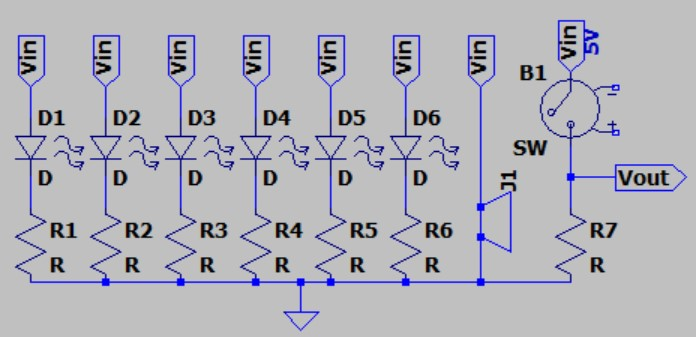
\includegraphics[width=1\textwidth]{skjema.jpg}
    \newpage

    \section{Oppgave}
        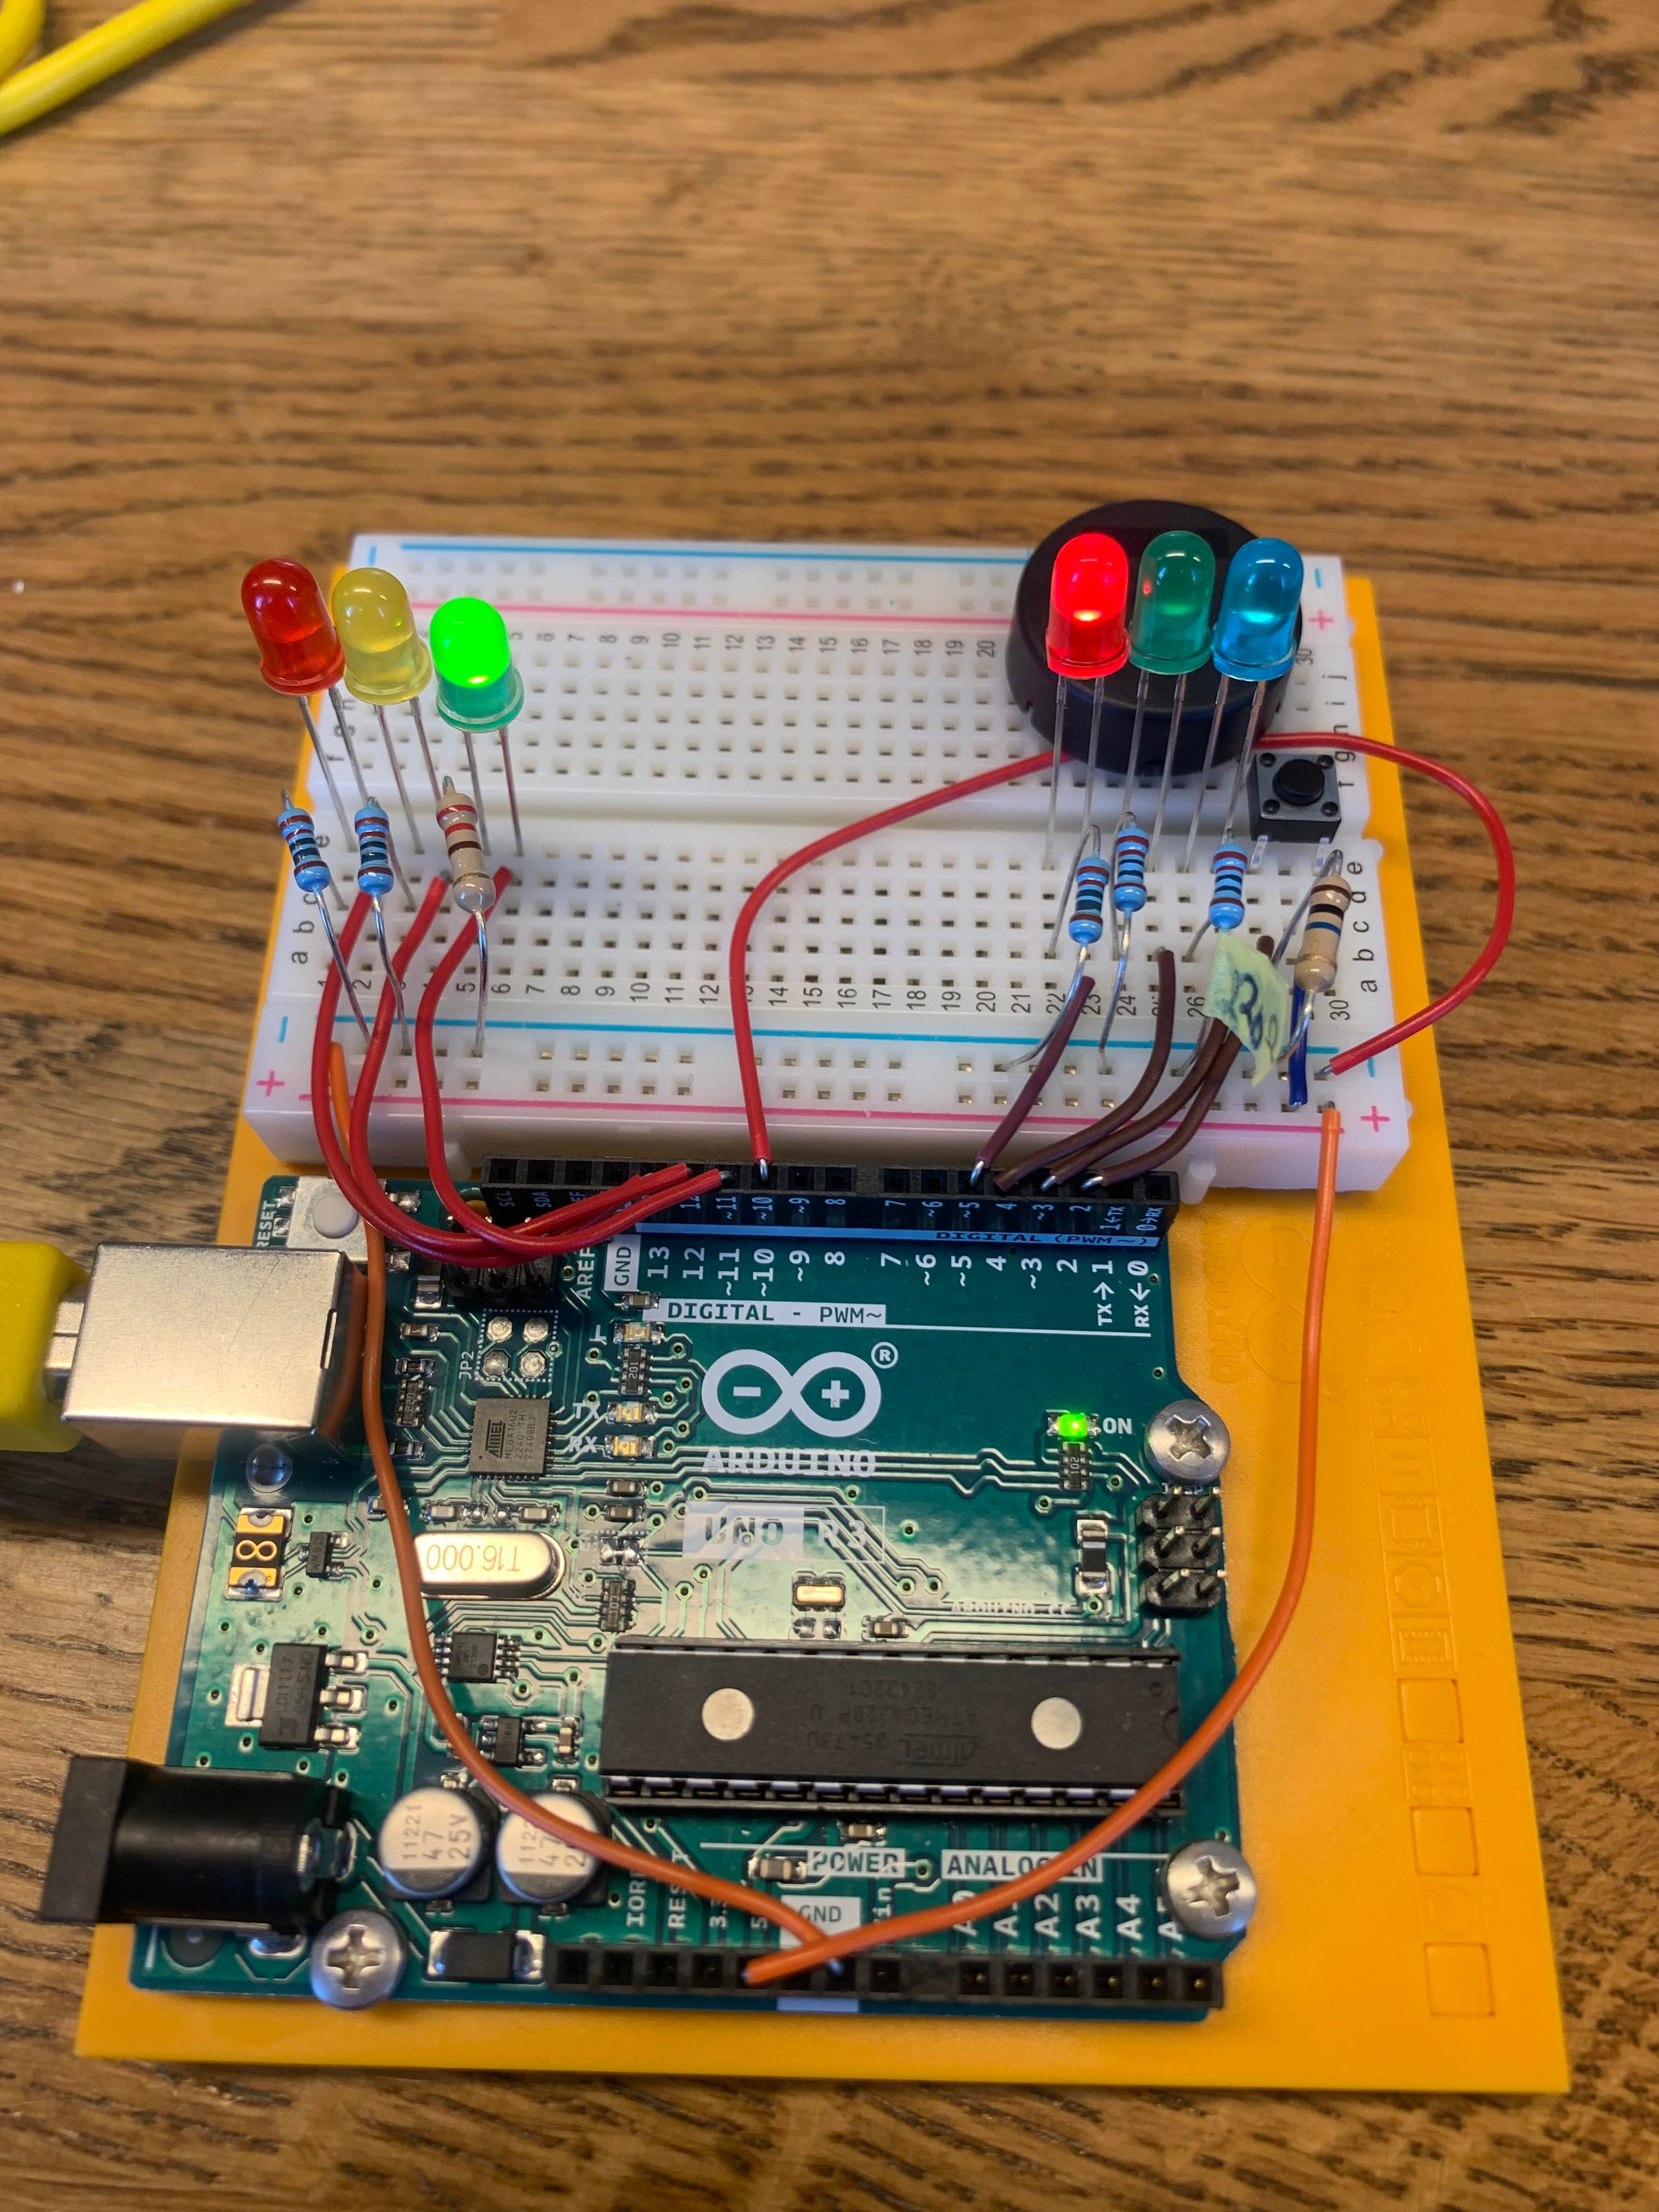
\includegraphics[width=1\textwidth]{oppsett_arduino.jpg}\\

\end{document}
